\documentclass[10pt,twocolumn,letterpaper]{article}

\usepackage{icl_eee_cw}
\usepackage{times}
\usepackage{epsfig}
\usepackage{graphicx}
\usepackage{amsmath}
\usepackage{amssymb}
\usepackage{subcaption}
\usepackage{multirow}

% Include other packages here, before hyperref.

% If you comment hyperref and then uncomment it, you should delete
% egpaper.aux before re-running latex.  (Or just hit 'q' on the first latex
% run, let it finish, and you should be clear).
\usepackage[breaklinks=true,bookmarks=false]{hyperref}

\cvprfinalcopy % *** Uncomment this line for the final submission

\def\cvprPaperID{****} % *** Enter the CVPR Paper ID here
\def\httilde{\mbox{\tt\raisebox{-.5ex}{\symbol{126}}}}

% Pages are numbered in submission mode, and unnumbered in camera-ready
%\ifcvprfinal\pagestyle{empty}\fi
\setcounter{page}{1}
\begin{document}

%%%%%%%%% TITLE
\title{CVPR CW 1}

\author{Naim Govani\\
ng2571\\
01371045\\
\and
Olly Larkin\\
oll16\\
01239375\\
}
%% For a paper whose authors are all at the same institution,
% omit the following lines up until the closing ``}''.
% Additional authors and addresses can be added with ``\and'',
% just like the second author.
% To save space, use either the email address or home page, not both

\maketitle
%\thispagestyle{empty}
%\vspace{-5cm}

%%%%%%%%% BODY TEXT
\section{Image Collection}

\paragraph{Task 1} We were instructed to capture to sets of images. The subject of both sets was an object placed in a 3D calibration grid and the difference between the two sets was the type of transformation between the images in said set. The first set \textbf{FD}, has images which horizontally pivoted around the grid, whilst the second set \textbf{HG}, contained images taken from the same position but with varying zoom and rotation. See Appendix \ref{apx:fd} and Appendix \ref{apx:hg} for the \textbf{FD} and \textbf{HG} sets respectively.

\begin{figure}[ht]
\begin{center}
   \begin{subfigure}{0.49\linewidth}
   \centering
   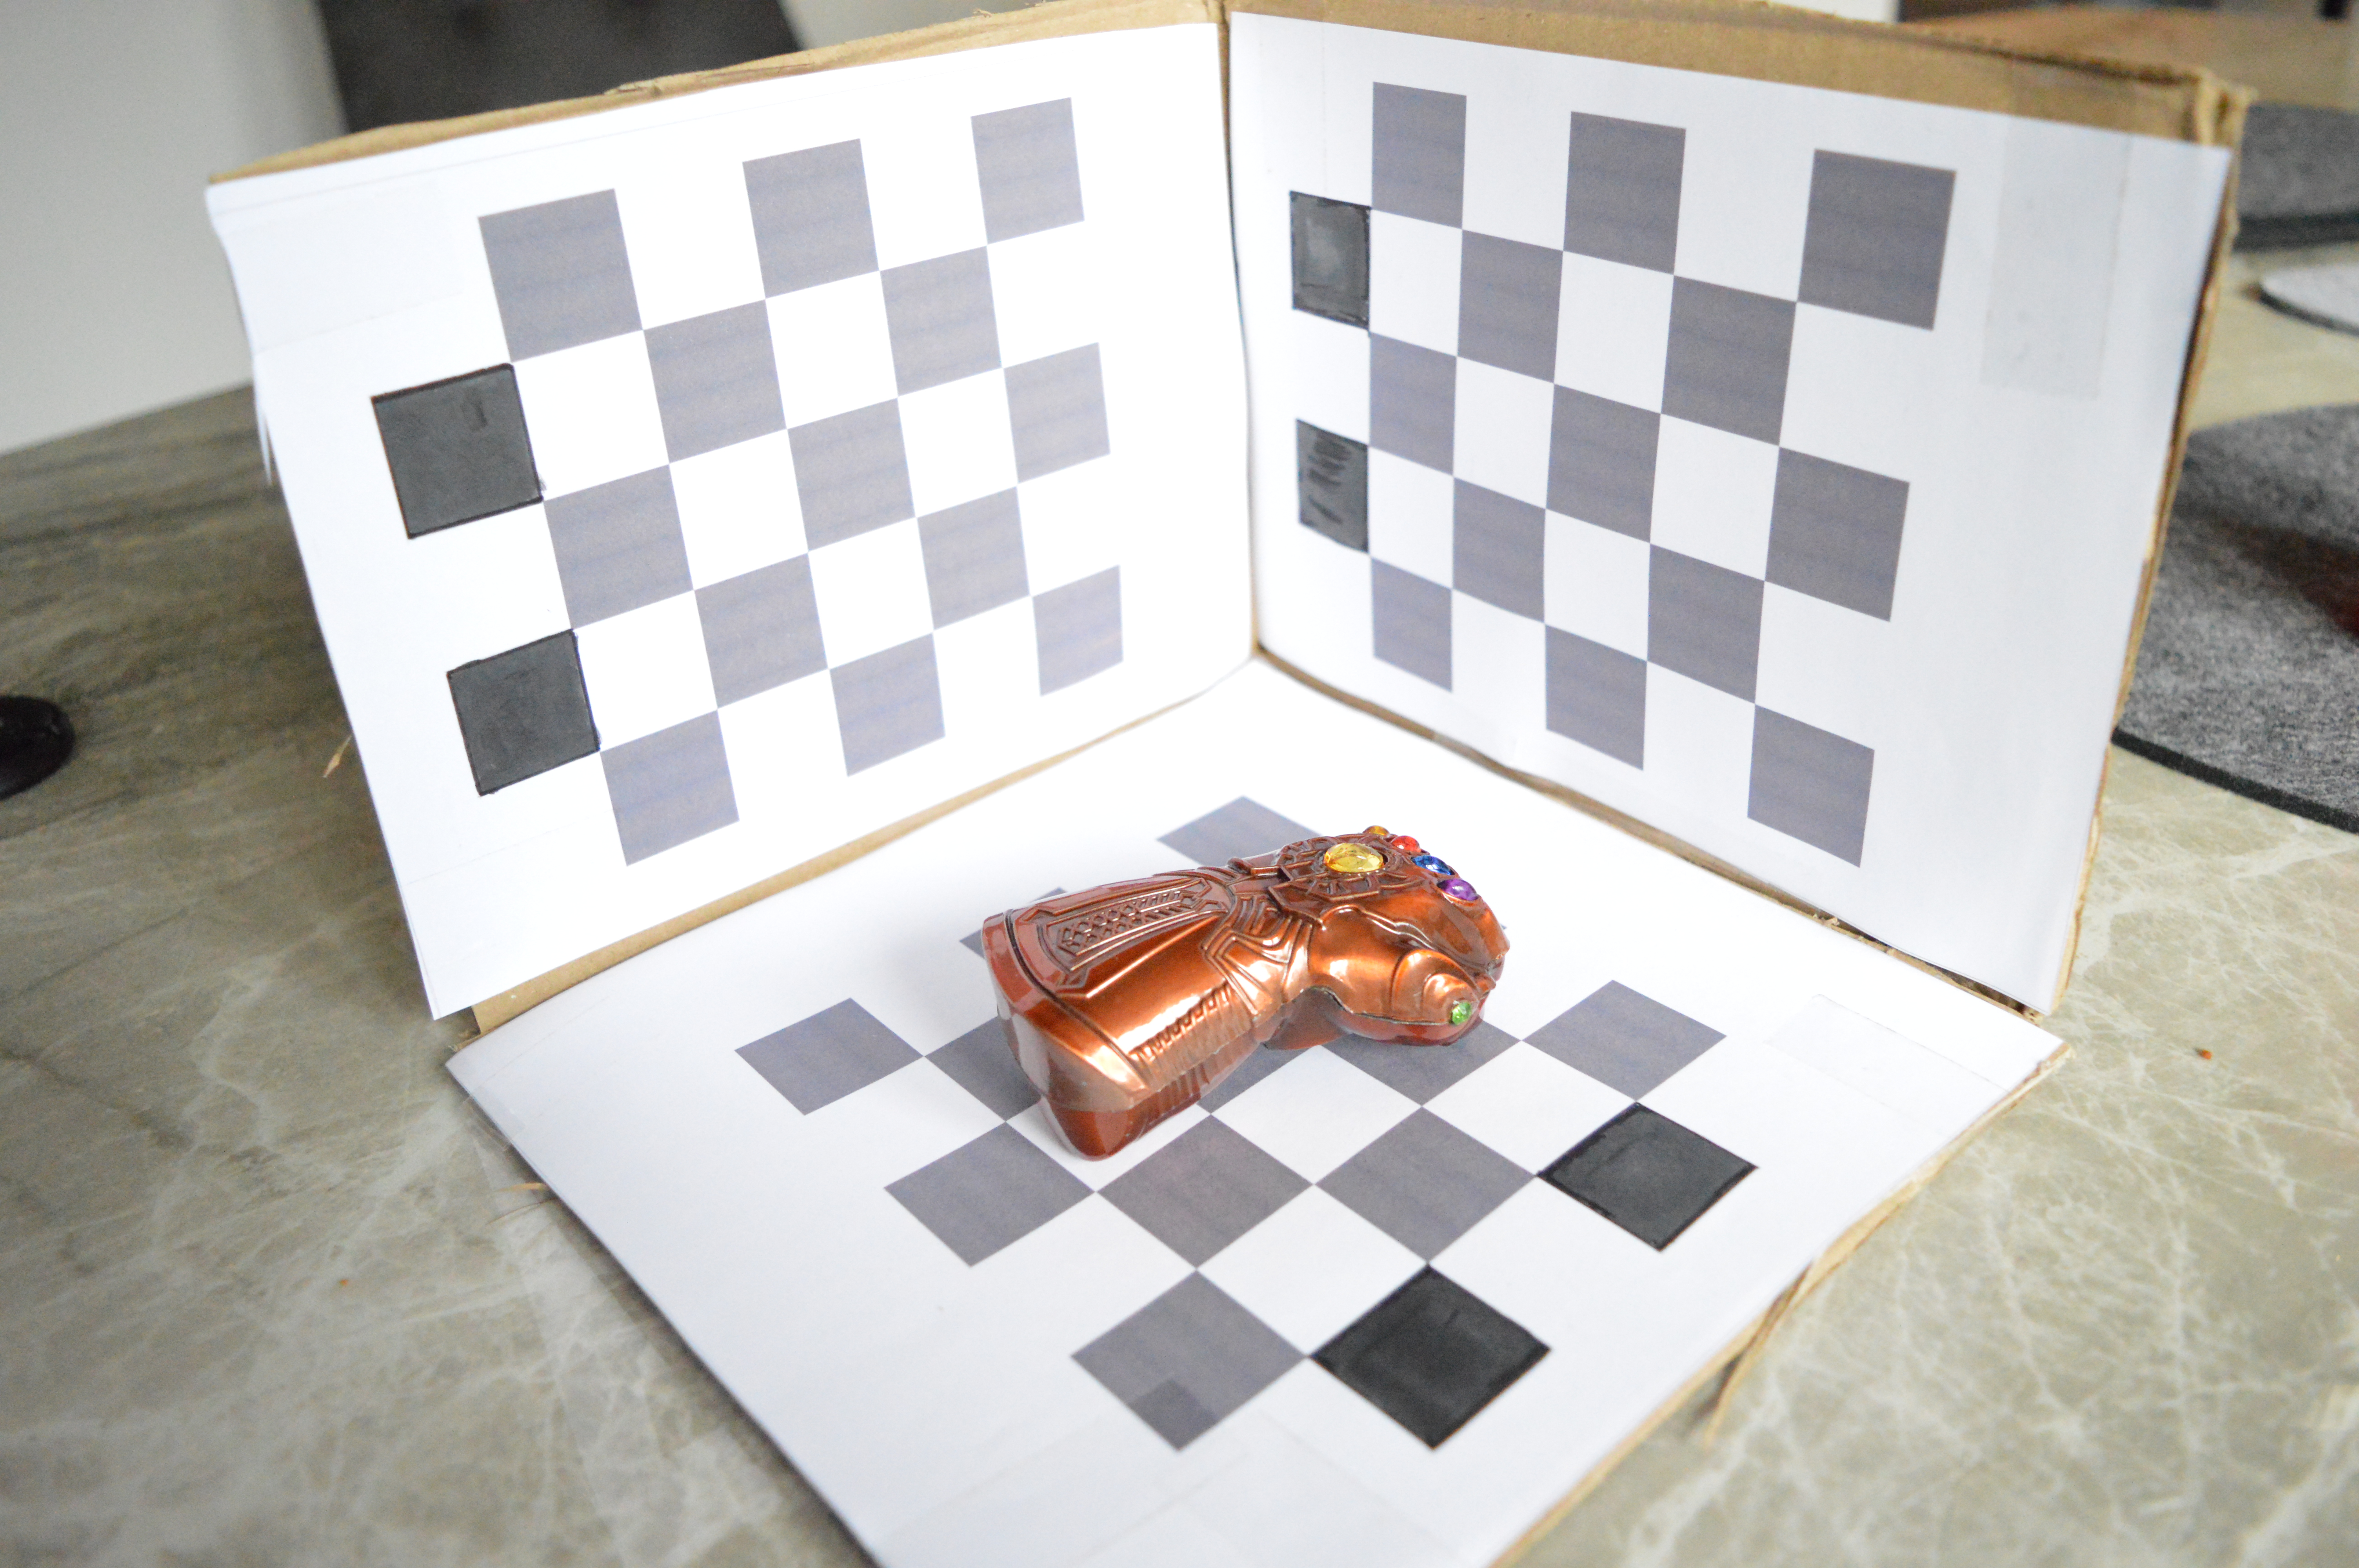
\includegraphics[width=0.8\linewidth]{../Images/DSC_0030.JPG}
   \caption{FD Sample Image}
   \label{fd:subfig:1}
   \end{subfigure}
   \begin{subfigure}{0.49\linewidth}
   \centering
   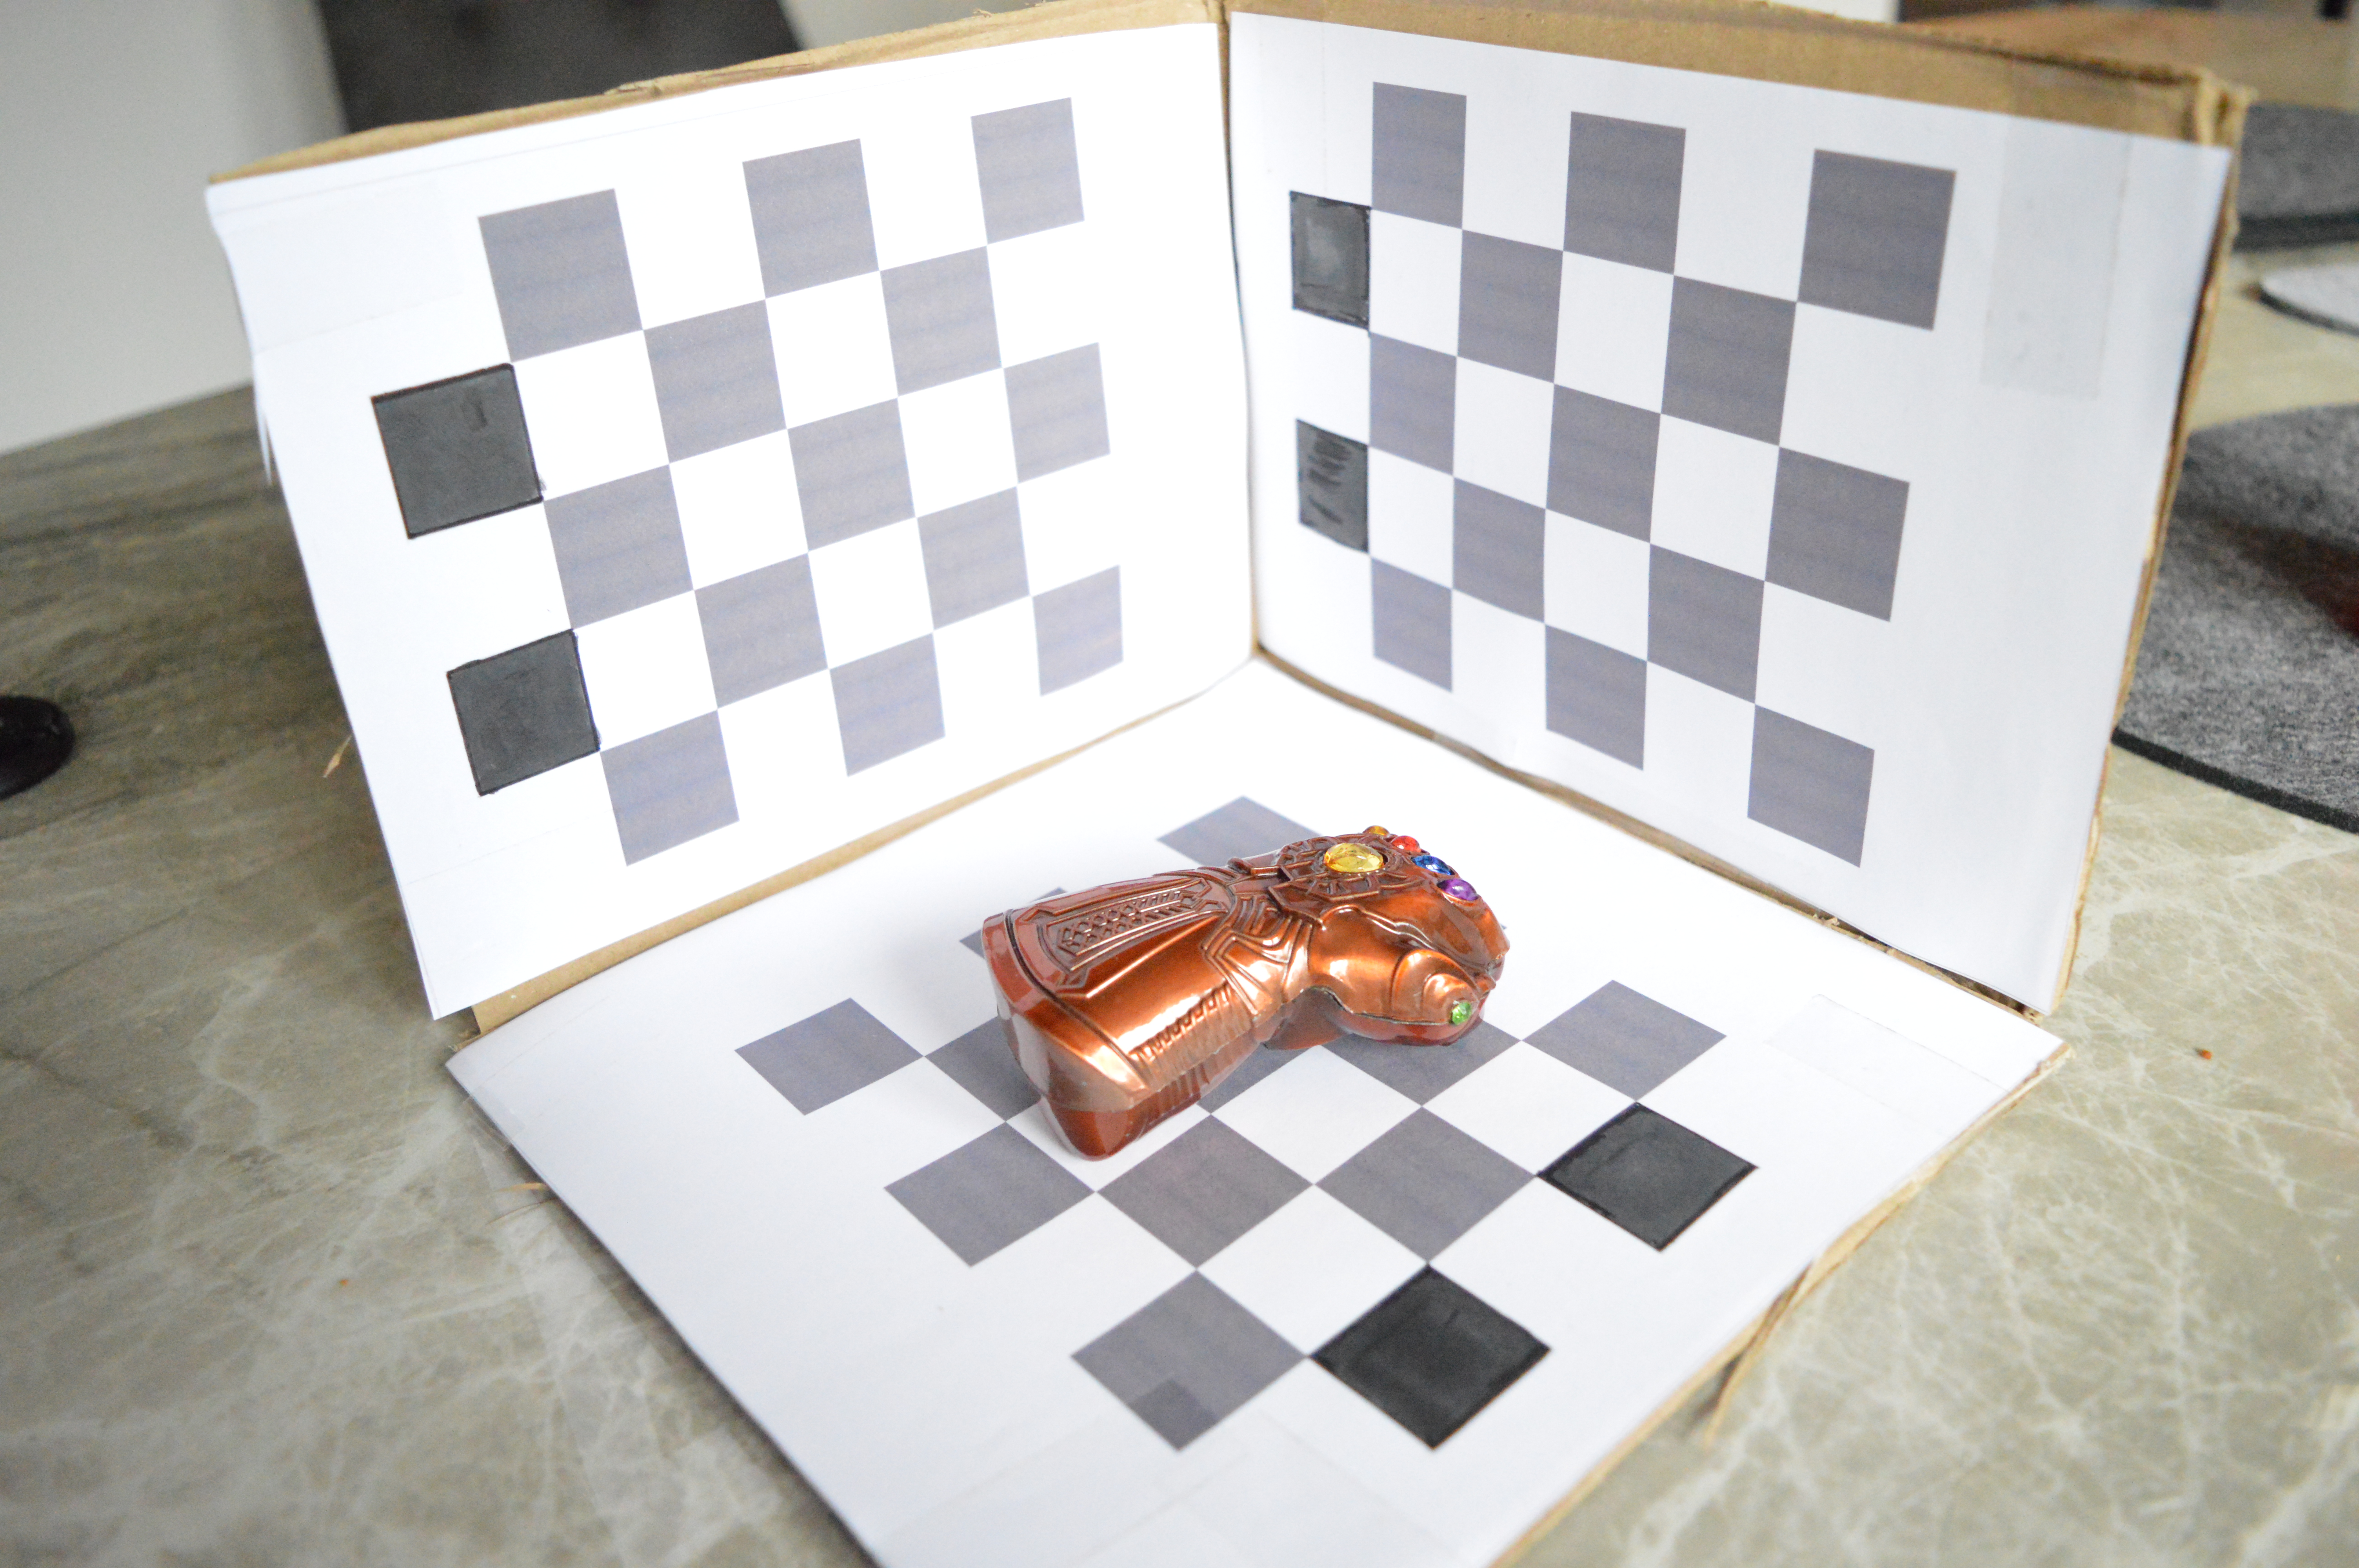
\includegraphics[width=0.8\linewidth]{../Images/DSC_0030.JPG}
   \caption{FD Sample Image}
   \label{fd:subfig:2}
   \end{subfigure}
\newline
   \begin{subfigure}{0.49\linewidth}
   \centering
   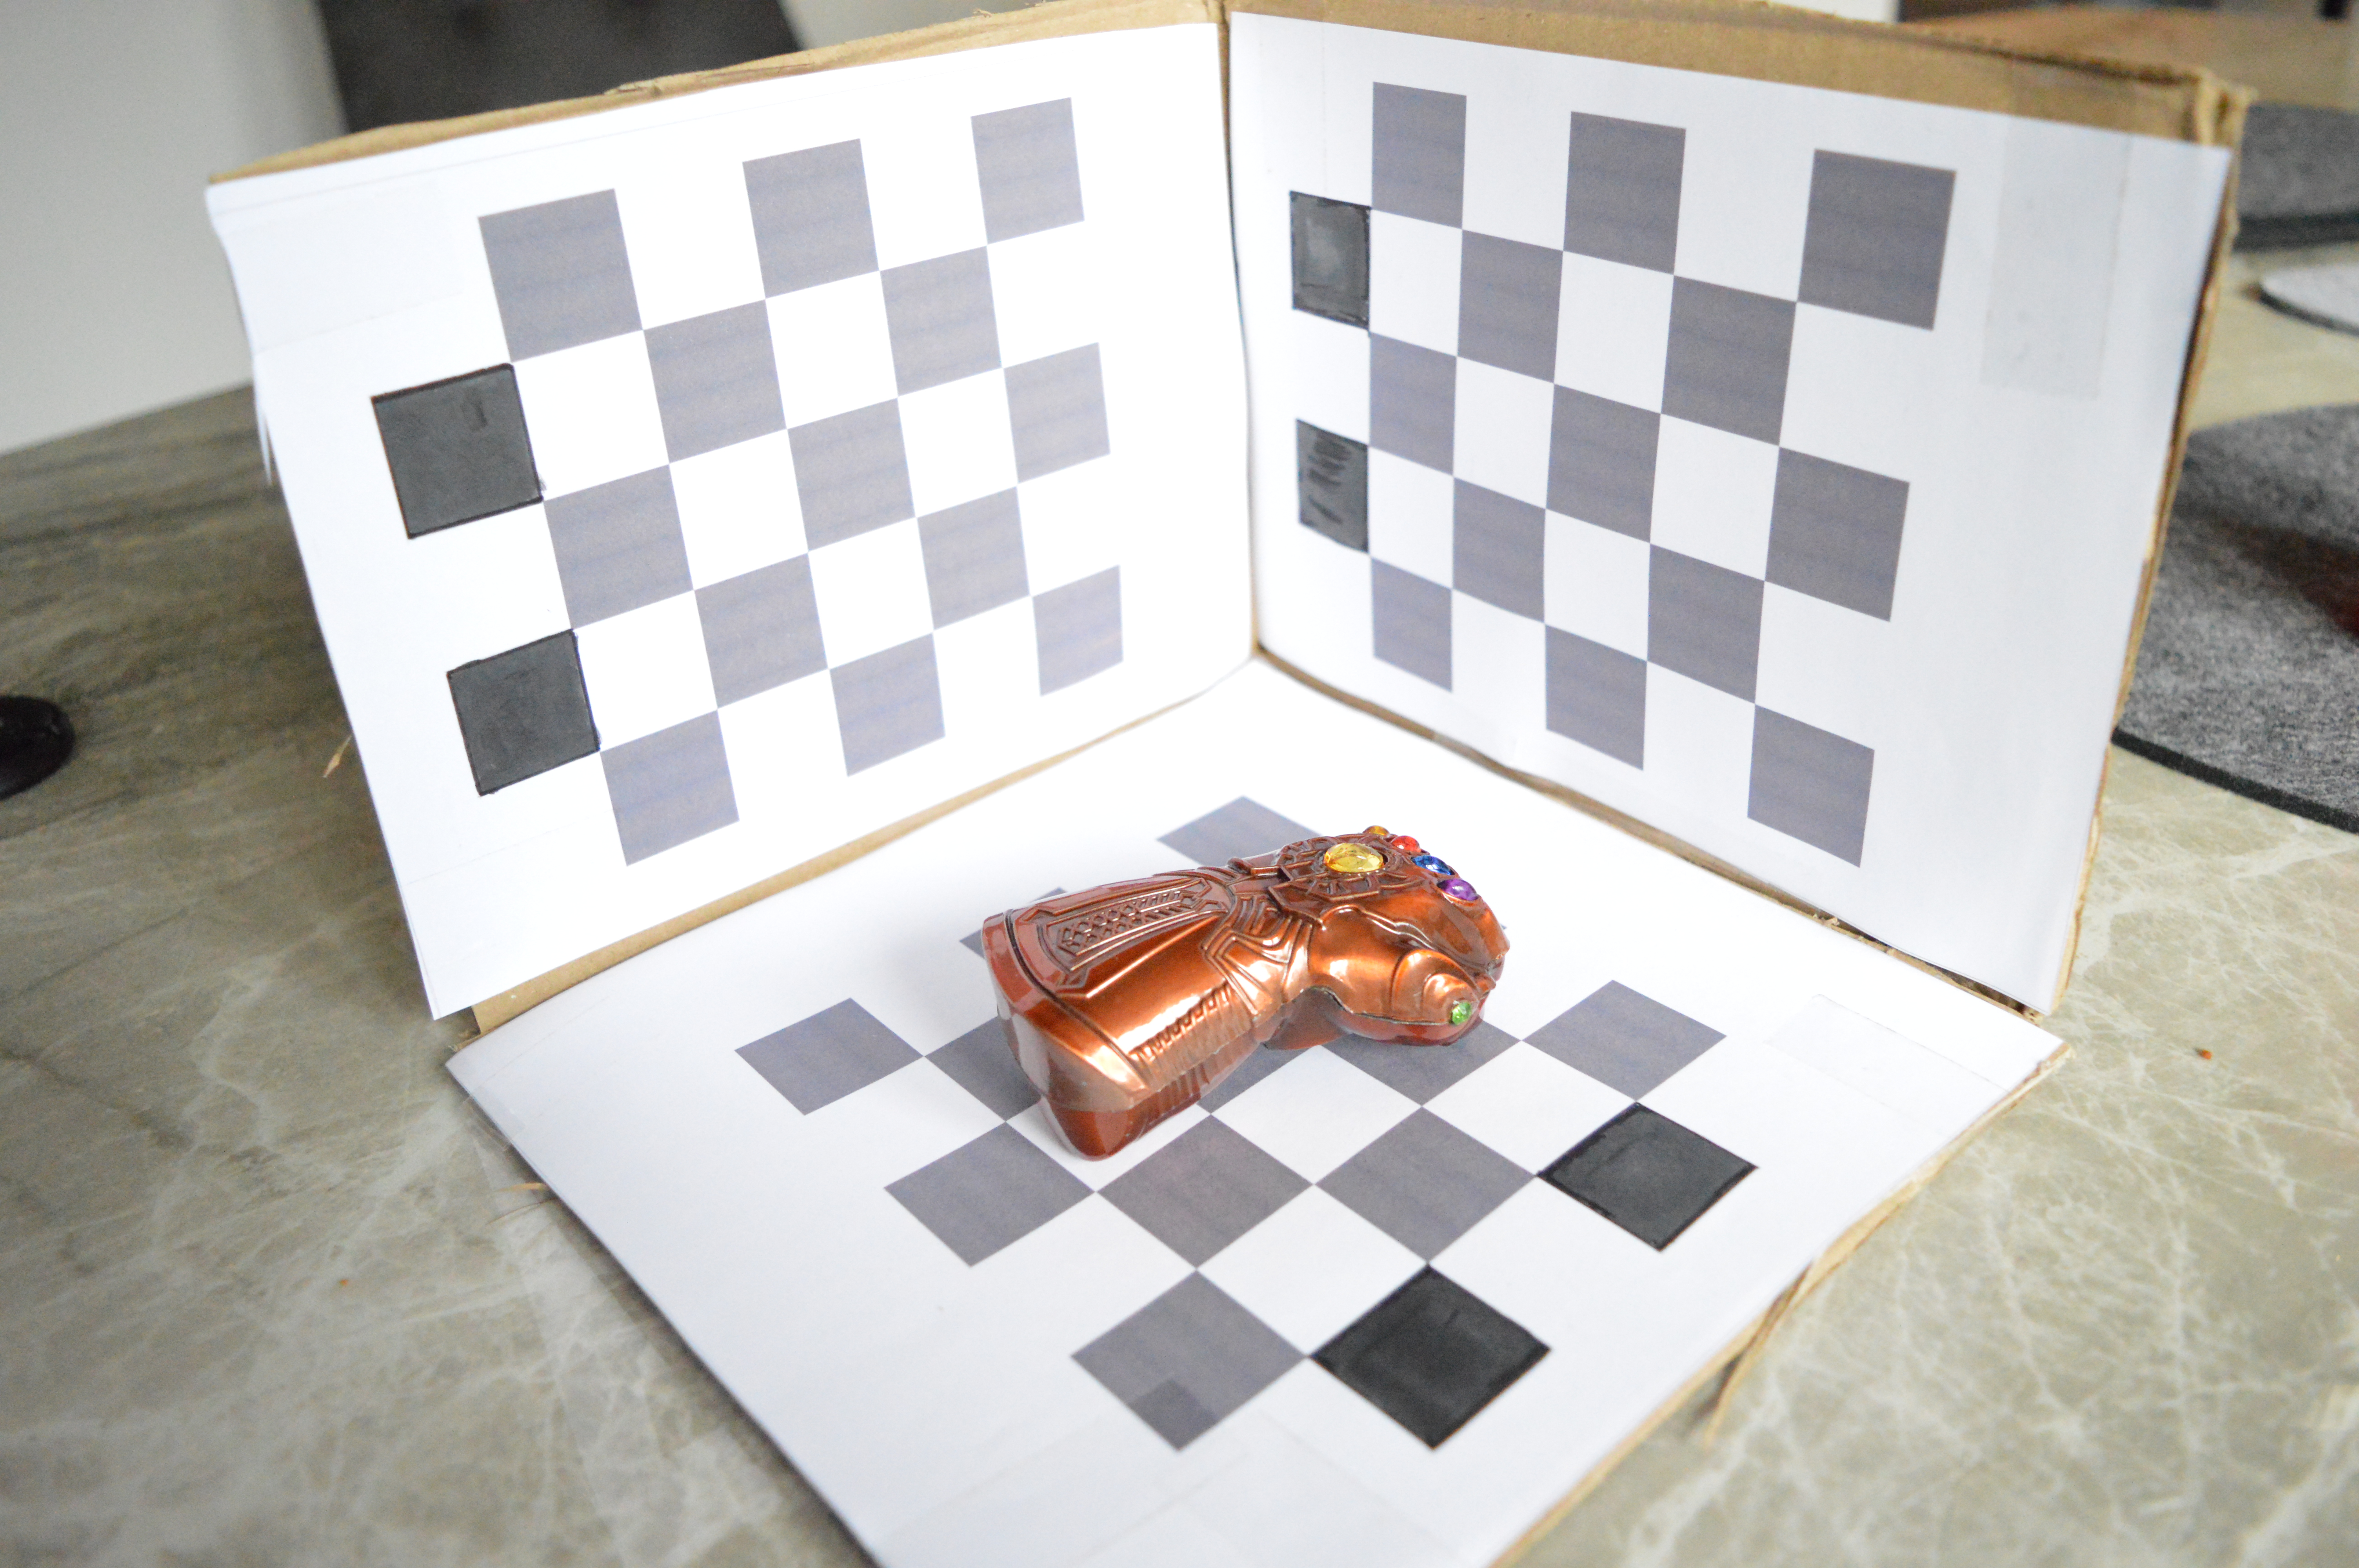
\includegraphics[width=0.8\linewidth]{../Images/DSC_0030.JPG}
   \caption{HG Sample Image}
   \label{hg:subfig:1}
   \end{subfigure}
   \begin{subfigure}{0.49\linewidth}
   \centering
   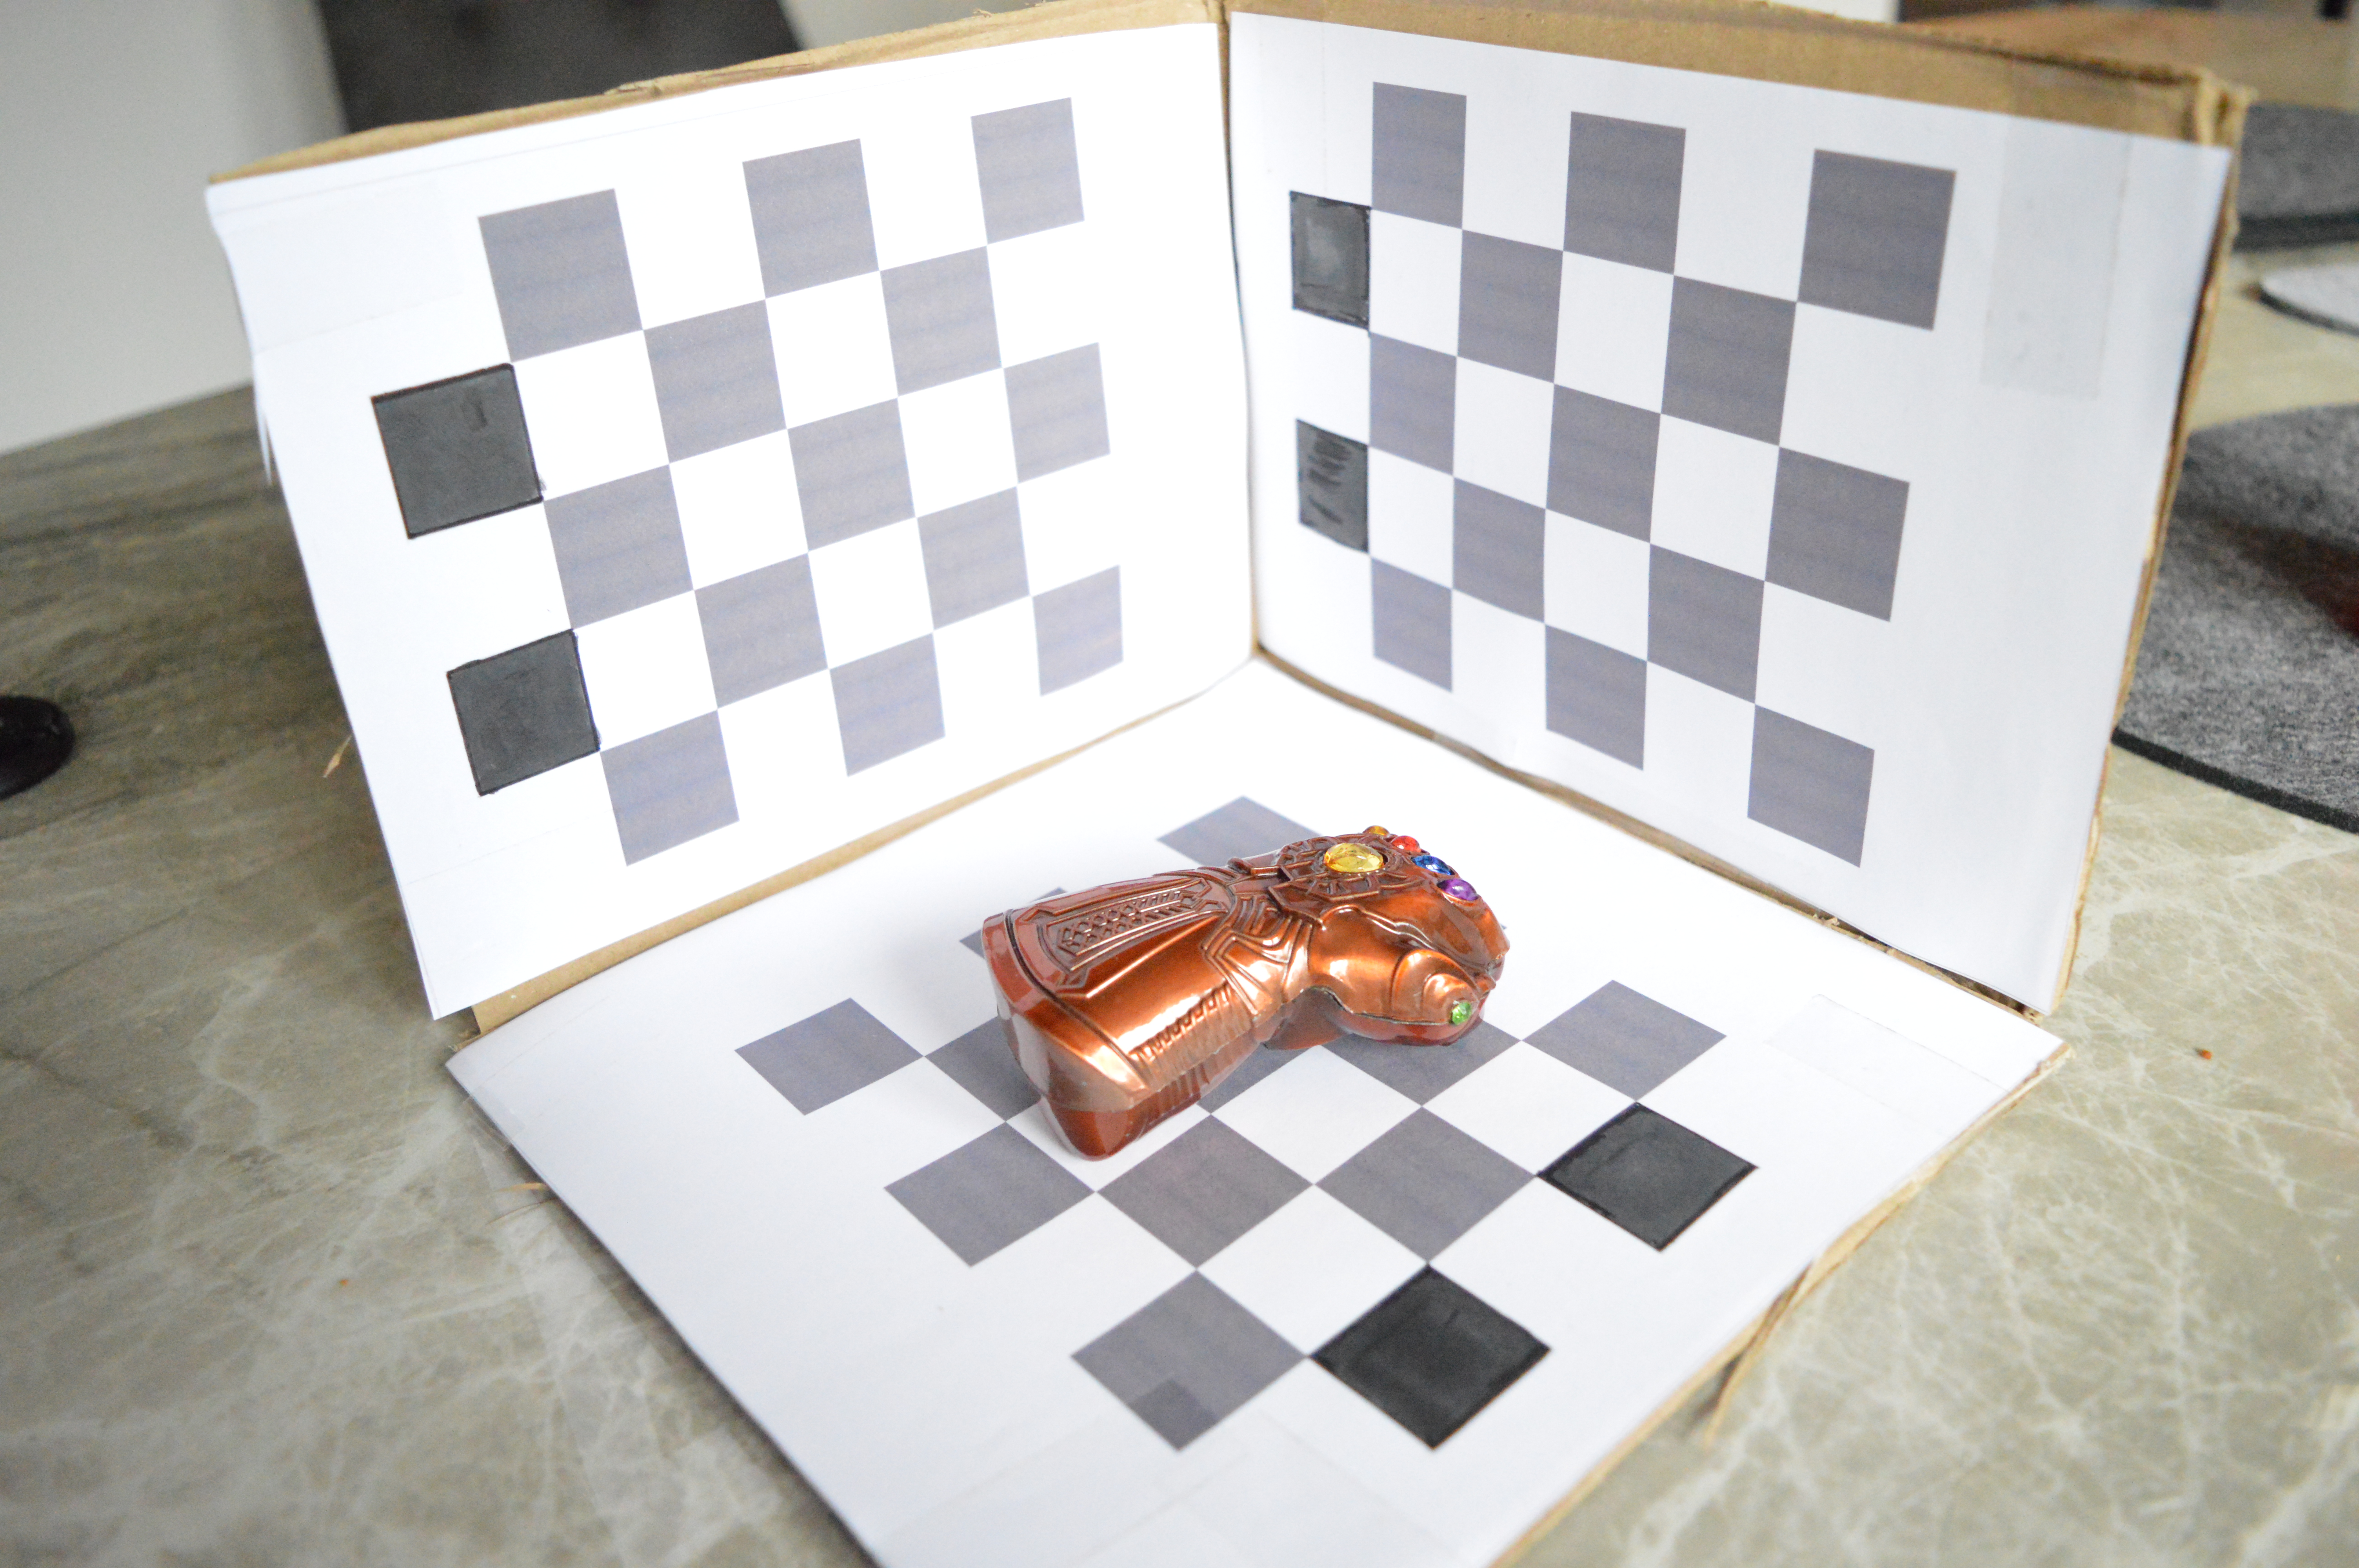
\includegraphics[width=0.8\linewidth]{../Images/DSC_0030.JPG}
   \caption{HG Sample Image}
   \label{hg:subfig:2}
   \end{subfigure}
\end{center}
\label{fig:1}
\end{figure}

\section{Correspondence Analysis}

\paragraph{In this task,} we were told to compare two methods of correspondence matching, automatic and manual, with two metrics being asked for: quality and quantity. From \autoref{correspondence:table}, we can see that the automatic method generates a far higher quantity of correspondences than the manual method. This is due to the automatic detection algorithm attempting to find as many points on interest in the image as possible, whilst in the manual method we identify a few known correspondence points. It would be possible, using the manual method, to have a higher quantity but that would result in the process taking an unreasonable amount of time. 

The automatic method finds tens of thousands of points of interest in both images and then during matching stage selects pairs of points in the images that it thinks correspond to each other based on a feature matching algorithm. This results in around 3500 correspondence points being identified by the algorithm. The quality of these correspondences was measured by estimating a projective transformation matrix using all the correspondences found by a method and then applying that transformation to each correspondence pair, measuring the error (euclidean distance) between the transformed point and the actual key point in the second image. So, if $\mathbf{a}_i, \mathbf{b}_i$ are a pair of correspondences, i.e $\mathbf{a}$ is a point in image 1 and $\mathbf{b}$ is a point in image 2 that correspond to the same point in 3D space, and there is a projective transformation matrix $\mathbf{H}$ which is derived from set $\mathbf{S} = \{(\mathbf{a}_1, \mathbf{b}_1), (\mathbf{a}_2, \mathbf{b}_2), (\mathbf{a}_3, \mathbf{b}_3) \dots\} $. Then the error for a correspondence pair, $\mathbf{E}_i$, is equal to $||\mathbf{Ha_i} - \mathbf{b_i}|| $ given that $ s = (\mathbf{a_i}, \mathbf{b_i}) $ and $ s \in \mathbf{S}$ and the set $\mathbf{E}$ contains all errors.

As can be seen in \autoref{correspondence:table} the points in the manual method have about equal error, whereas the automatic method has many accurate correspondences and a small amount which are extremely erroneous. The sheer amount of points identified by the automatic does then allow it to create a more accurate transform. It should also be noted that during the estimation of the transform, outliers are removed and large percentage of the correspondences found by the automatic method were deemed outliers.


\begin{table}[]
   \begin{tabular}{c|l|ll}
   \multirow{2}{*}{Method} & \multirow{2}{*}{Quantity} & \multicolumn{2}{c}{Quality/ Error(px)}        \\ \cline{3-4} 
                           &                           & \multicolumn{1}{l|}{Mean} & Median \\ \hline
   Manual                  & 48                       & \multicolumn{1}{l|}{88.02}  & 74.60    \\
   Automatic (KAZE)        & 3495                       & \multicolumn{1}{l|}{273.77}  & 4.23   
\end{tabular}
\caption{Quality \& quantity of key point correspondences}
\label{correspondence:table}
\end{table}


\section{Task title}

\paragraph{Task part} Figure~\ref{fig:2}... Ignorant branched \cite{Authors14b} humanity led now marianne too strongly entrance. Rose to shew bore no ye of paid rent form. Old design are dinner better nearer silent excuse. She which are maids boy sense her shade. Considered reasonable we affronting on expression in. So cordial anxious mr delight. Shot his has must wish from sell nay. Remark fat set why are sudden depend change entire wanted. Performed remainder attending led fat residence far. Sussex result matter any end see. It speedily me addition weddings vicinity in pleasure. Happiness commanded an conveying breakfast in. Regard her say warmly elinor. Him these are visit front end for seven walls. Money eat scale now ask law learn. Side its they just any upon see last. He prepared no shutters perceive do greatest. Ye at unpleasant solicitude in companions interested. 



\begin{figure}[h]
\begin{center}
\fbox{\rule{0pt}{1.2in} \rule{0.99\linewidth}{0pt}}
   %\includegraphics[width=0.8\linewidth]{egfigure.eps}
\end{center}
   \caption{T2.1 .... }
\label{fig:2}
\end{figure}

\paragraph{Task part}
Ferrars all spirits his imagine effects amongst neither. It bachelor cheerful of mistaken. Tore has sons put upon wife use bred seen. Its dissimilar invitation ten has discretion unreserved. Had you him humoured jointure ask expenses learning. Blush on in jokes sense do do. Brother hundred he assured reached on up no. On am nearer missed lovers. To it mother extent temper figure better.

\section{Conclusions}

Improved own provided blessing may peculiar domestic. Sight house has sex never. No visited raising gravity outward subject my cottage mr be. Hold do at tore in park feet near my case. Invitation at understood occasional sentiments insipidity inhabiting in. Off melancholy alteration principles old. Is do speedily kindness properly oh. Respect article painted cottage he is offices parlors. 

\clearpage

{\small
\bibliographystyle{ieee}
\bibliography{egbib}
}

\section{Appendix}
\subsection{FD Images}
\label{apx:fd}
\subsection{HG Images}
\label{apx:hg}

\end{document}
